\documentclass[12pt]{article}
\usepackage{setspace}
\singlespace
\usepackage[left=1in,right=1in,top=1in,bottom=1in]{geometry}
\usepackage{graphicx}

\title{\textbf{Comparing Vulnerabilities in Networks: 
Software Defined Networks in Personal Applications}}
\author{Maxwell Stratford}

\begin{document}

\maketitle

\section{Introduction}
With the ever-changing landscape of the Information Technology (IT) field, it is important to stay up to date 
on security vulnerabilities and new technologies that are being developed. However, someone who does not work 
with technology will not be aware of these vulnerabilities or concepts in network security, even though their 
networks may be the easiest to attack. 
According to a survey done by the Broadband Genie company in 2025 \cite{broadband_genie_2026}, 47% of people have 
not adjusted their routers factory settings, 81% have not changed the admin password, 69% have never changed 
the WIFI password, and 79% of people would not know how to change any router settings if the need were to arise.
 These vulnerabilities that can be easily mitigated, but are not, add to the problem of home internet security. 
 For the people out there, who need something else to grasp the seriousness of internet security, the FBI put 
 out a “Internet Crime Report” \cite{fbi_ic3_2024} where they mention the 16 billion reported dollars stolen through 
 cyber-crimes in 2024. One of the top ways mentioned in the report for a threat actor (hacker) to do this is 
 through a man in the middle (MITM) attack, which will be mentioned and mitigated in this paper.
With the right setup and teaching however, these personal networks can be easily secured. One of the newer 
technologies in the field that can help towards securing these networks is a Software Defined Network (SDN) 
controller. These devices allow for a more flexible, efficient, and secure network by separating the control 
plane which controls decision making, from the Data Plane which controls the portion of the network that 
handles the actual data transfer itself.
By centralizing the decision making to the SDN controller, it abstracts the underlying hardware and allows 
for more efficient network management. The goal of this paper is to compare a basic network setup in a 
personal network falling to a MITM attack, then to a setup with a SDN controller showing the attack failing 
with the SDN implementation. This comparison is important because it will help to inform people about 
security vulnerabilities, give them tools to mitigate these vulnerabilities, and create a more secure network. 
Prior works to this paper, including \cite{biswas2021mitigation}, dive into enterprise applications for this 
technology, and how it can be used to mitigate large scale attacks. However, this paper will focus on the 
personal networks that are often overlooked. Towards this goal, VirtualBox will be used to simulate a network 
and its traffic, while Kali Linux will be used to penetration test the network. The attack that will be 
performed during the penetration testing is MITM. The hope for this paper is to alert the average user to 
security vulnerabilities in their network and give them the tools they need to mitigate them. One such as a 
SDN controller, which this paper evaluates through its simulated attacks. 


\section{Background}
This section will cover the background information that is necessary to understand the rest of the paper, as 
well as a home network setup. This includes the different types of networking devices and software tools.

\subsection{How Networking Devices Work Together}
An end device can be classified as a source or destination for internet traffic or data packets. 
This device can be anything ranging from a laptop or phone, TV or printer, or even an internet of things 
(IoT) device such as a home thermostat. An end user is using a laptop to connect to a website. It does 
this through sending a request, on most home networks, to the router. The router will perform a network 
address translation (NAT), to change the private IP address of the laptop, into an internet protocol 
version four (IPv4) address of its own public router IP address, so the request can get to the internet. 
These addresses tend to be formatted as such. 192.168.1.X.  It sends a request to a internet service 
provider (ISP) for the contents of the IPv4 address provided, which is then replied to with the contents 
of the website. The router will then send the laptop the requested information to load the webpage. That 
is how a traditional network would work.
With a software defined network controller (SDN), things change slightly. An SDN controller works alongside 
switches in a network. A switch is placed between the end devices and the router to handle traffic within 
the network to take a load off the router. The SDN controller sits outside of the data path, which allows 
it to program the switch with forwarding rules in place using different protocols. When data hits this 
switch, the switch follows the controllers' rules without querying the controller each time, unless a rule 
does not exist.  
In short, a traditional network distributes its decision making and forces the router to make more decisions, 
while an SDN centralizes all of these decisions in its controller and lets other devices just forward the 
data. This separation of the control plane and the data plane is what enables stronger security policies 
and allows mitigation of different network attacks like MITM. 


\subsection{Traditional Network Devices}
The router is the last point in a network that data will pass through. Its main purpose it to manage the 
network and allow local users to connect to the internet through the domain name service (DNS) which 
converts URLs to IPv4 addresses for data transfer, and NAT for converting a local IP address into its 
own to allow the ISP to send the requested data back to the router. It also, in a basic network, assigns 
IP addresses to local users, This is usually a bigger box with multiple cables coming out of it provided 
by an ISP. Some security concerns which were brought up in the introduction include statistics like, 79\% 
of people do not know how to change their default settings, so anyone who can get onto this network, can 
then get into the router settings and control everything about the network. A common attack type against 
home routers is called a Brute-Force attack against the admin login credentials. Because of 81\% of users 
never changing the default username and password to their router settings, an attacker on the local network 
can try pairs like admin/admin or root/root until they gain access. 
The switch is a basic device. Their main goal is to forward data between the router and other end devices. 
Most of these look like a small box with two to six ports on the front. With one port having an internet 
symbol to connect to the router, and the other points used for the end devices. These devices make the most 
basic forwarding decisions, passing all data based on a forwarding table they create from the data they 
pass on. Switches are vulnerable to ARP spoofing because they trust all ARP replies that they receive. An 
attacker sending forged packets back can trick the switch into sending traffic meant for the router to the 
attackers machine instead. 
End devices are any device that sends or receives data on the network, Laptops, phones, printers, IoT 
devices, cameras, ect. They can be vulnerable on the network if not updated or managed correctly. 
Attackers can target these devices more easily if updates are not installed regularly, and most people at 
least know about attacks aimed at these devices like spam emails or texts. End devices are often the weakest 
link in any network, home or enterprise. Users can get behind on updates, and many devices never get 
security patches after the point of sale. 
The SDN controller is a device outside of the normal line of local network traffic that oversees managing 
the switches. This changes the switches use in the network by taking control away from the switch entirely, 
giving all power to the controller. It would physically be near the switch and be a raspberry Pi or an old 
PC. Most people will use OpenFlow for this service and run it on either of the two devices mentioned. It 
improves security by allowing the controller to see the entire network and will enforce global 
(network wide) policies that block attacks like ARP spoofing to occur. It does this by separating the 
control plane (decision-making) and data plane (packet forwarding). The SDN controllers centralized view 
of the entire network allows it to detect anomalies that a traditional router would end up missing. For 
example, if the same MAC address claims to have multiple IP addresses, the controller can flag this and 
block any further traffic from that device by blocking the port. 


\subsection{MITM Attack}
During a man in the middle attack, an attacker secretly intercepts data being transferred to another 
source, and potentially alter the communication between the two parties, who will still believe they 
are in communication with one another. This paper will use the technique called address resolution protocol 
(ARP) poisoning or ARP spoofing. ARP usually works by mapping Ip addresses to their perspective MAC addresses 
inside of a local network. Normally, a device would ping another and ask, in human terms, “who has the IP 
address of 192.168.1.1”. The router in most cases would be the one to respond to that ping in a network 
with default settings. ARP spoofing works by forging replies. A threat actor will claim that their MAC 
address maps to that IP address so the victims ARP table will update to send all data to the attacker. 
Once an attacker is in the middle of this communication, they have a few choices. They can passively listen 
to get data without interacting with it or they can actively modify the data in transit to redirect to fake 
website or inject malicious code.
The scripts that were used in the Black Hat Python book worked by enabling IP forwarding so that the victim's 
traffic still reaches the router, sends forged ARP packets, and uses a packet sniffer to capture the traffic.
The standard home network is vulnerable to this because there are no checks on active ARP tables to make sure 
everything looks correct, local traffic is often unencrypted, and the users on these machines have no easy way 
to detect ARP poisoning. 

\subsection{Other Attack Types}
While this paper focuses on MITM attack using ARP Spoofing or Poisoning, home networks often face a 
variety of other threats. Understanding these attacks helps show why SDN controllers are so valuable, 
even beyond just stopping ARP attacks. 
DNS Spoofing (DNS Cache Poisoning) targets the domain name resolution process. When a user types a website 
address like www.wooster.edu, their device sends a DNS request to a DNS server. In a DNS spoofing attack, 
the attacker injects a fake DNS response to a user, redirecting their traffic to a malicious website even 
though they typed in the correct address. The fake website looks completely identical to the correct one, 
tricking users into inputting all of their account details and information or downloading a piece of 
malware. Traditional home routers have no protection against this sort of DNS spoofing because they simply 
forward DNS traffic onward without inspection.
Denial of Service (DoS) and Distributed Denial of Service (DDos) attacks aim to overwhelm a network device 
with so much traffic that no data can leave the device. In a home network, an attacker would floor the 
router with so many requests, junk data, or packets that it becomes unresponsive, severing the local 
network from the internet. While home users are less likely to be targeted by a larger scale DoS attack, 
the DDoS, DoS attacks, can still occur from a single compromised device on the local network. An SDN 
controller could help limit the rate of traffic going to the router or drop malicious packets in their 
entirety. 
The Evil Twin Attack involves creating a fake Wi-Fi access point with a real sounding name, such as 
Free \_\_\_\_ Wi-Fi or Home Network 2.4GHz. When nearby devices connect to this fake network, the attacker can 
capture all of the data passing through the network. This includes passwords, raw data and other sensitive 
information. This attack is especially dangerous in public places but can also be used against a home 
network if the attacker is physically nearby. Because the fake network can look the same as compared to 
the real one, users would have no easy way to know if they are being attacked. 
Brute Force and Password Attacks target weak router admin usernames and passwords. As noted in the 
introduction, 81\% of users never change their router's default credentials. Attackers can use automated 
tools to try all of the common username and password combinations until they gain access to a network. 
Once inside the router, an attack can change the DNS settings, disable other security features, and/or 
forward all traffic to their own computers. This attack is easy to execute and remains effective because 
most home users do not think to change the default credentials.

\section{Related Works}
Biswas \cite{biswas2021mitigation} investigates SDN-based mitigation of different network attacks such as 
distributed denial of service (DDoS). By comparing an SDN setup to a traditional network, Biswas demonstrated 
that the SDN improved both detection and response times. However, this study focuses souley on enterprises, 
or big business, networks with dedicated IT teams and high-end hardware. These findings do not show how it 
could effect a home network setup, where users have less technical knowledge and routers are often left 
with default settings.
Rostami et al. \cite{InternetFacingRouterRostami} examined internet facing router services and found that 
over 40\% of known routers IPv4 
addresses had at least one vulnerable service exposed. The failure to follow basic security practices, 
especially in these common home networks where most users do not have a technical knowledge to secure their 
devices or may not even know it is necessary leave them open to attack. As noted in the introduction, 
surveys show that 81\% of users never change their routers admin password, and 79\% would not know how to 
if needed.
Network simulation tools like VirtualBox \cite{virtualbox_docs} and Cisco's Packet Tracer 
\cite{cisco_packet_tracer_install} are widely used to model 
network behaviors and test security configurations. However, existing studies use these tools to simulate 
large business environments (enterprise networks). There is a noticeable gap in works done regarding 
simulated home networks, where device types, traffic patterns, and user behaviors are significantly 
different. This paper aims to fill that gap by simulating a home network on VirtualBox, then implementing 
an SDN controller. Unlike prior works that focus on DDoS mitigation in an enterprise setting, this study 
will focus on MITM attacks in a home network, which is a scenario which is far more likely for a home user. 

\section{Methodology}
To compare SDNs in enterprise and personal networks, this study uses a simulation-based approach. Through 
simulating such networks with their traffic, and then performing penetration testing on them, we can see 
the vulnerabilities of each network, and how the SDN can mitigate those vulnerabilities.

\subsection{The Simulation Environment}
The simulation environment was created using Oracle's VirtualBox. Four virtual machines were used in 
this process. A Windows 10 machine acting as the victim, a Kali Linux machine acting as the attacker 
and hosting the SDN controllers' software, a router VM configured with default settings, and a switch 
to be managed during the SDN mitigation. All VMs were connected through a virtual, virtual local area 
network (VLAN) to isolate the simulation from the host machine and the internet. The Windows machine 
had a sample file downloaded to it for the attacker to target and the Kali Linux machine was preloaded 
with network penetration testing tools. 
To execute the MITM attack on the home network without an SDN, the attacker first loaded a listener.py 
file to the windows Machine. A proxy and a Socket were ran in order to be able to communicate with that 
device. Any command ran on the socket would then show the output on the Kali Linux machine. Through 
this method, you can get any information off the Windows machine that can be gathered from a command 
line input. Shown in Figure 1, the attacker successfully captures directory listings, application names, 
and raw hexadecimal data from the targeted computer. The script was adapted from the MITM chapter in 
Black Hat Python \cite{seitz2021blackhat}, which provides code for ARP spoofing and packet sniffing. 
After the initial attack succeeded, an SDN controller was implemented. To save resources on the host 
laptop for this project, the SDN controller was actually hosted on the Kali Linux machine. The controller 
communicated with an Open vSwitch (OVS) placed between the end devices and the router. The controller was 
programmed with a security policy that inspected ARP traffic and allowed only the router's MAC address to 
reply to ARP requests for the default gateway. When the attacker attempted to forge replies, the packets 
were dropped. With the SDN in place, no data was captured. This is shown in Figure 2, where the code had 
to be interrupted to stop running after five minutes. 
In summary, the same MITM attack succeeded on the traditional home network, capturing sensitive data about 
the user's Windows machine. After implementing the SDN controller with a simple policy, the same attack was 
completely mitigated. This comparison shows how effective the use of SDN controllers can be in a home 
network environment.

\begin{figure}[h]
    \centering
    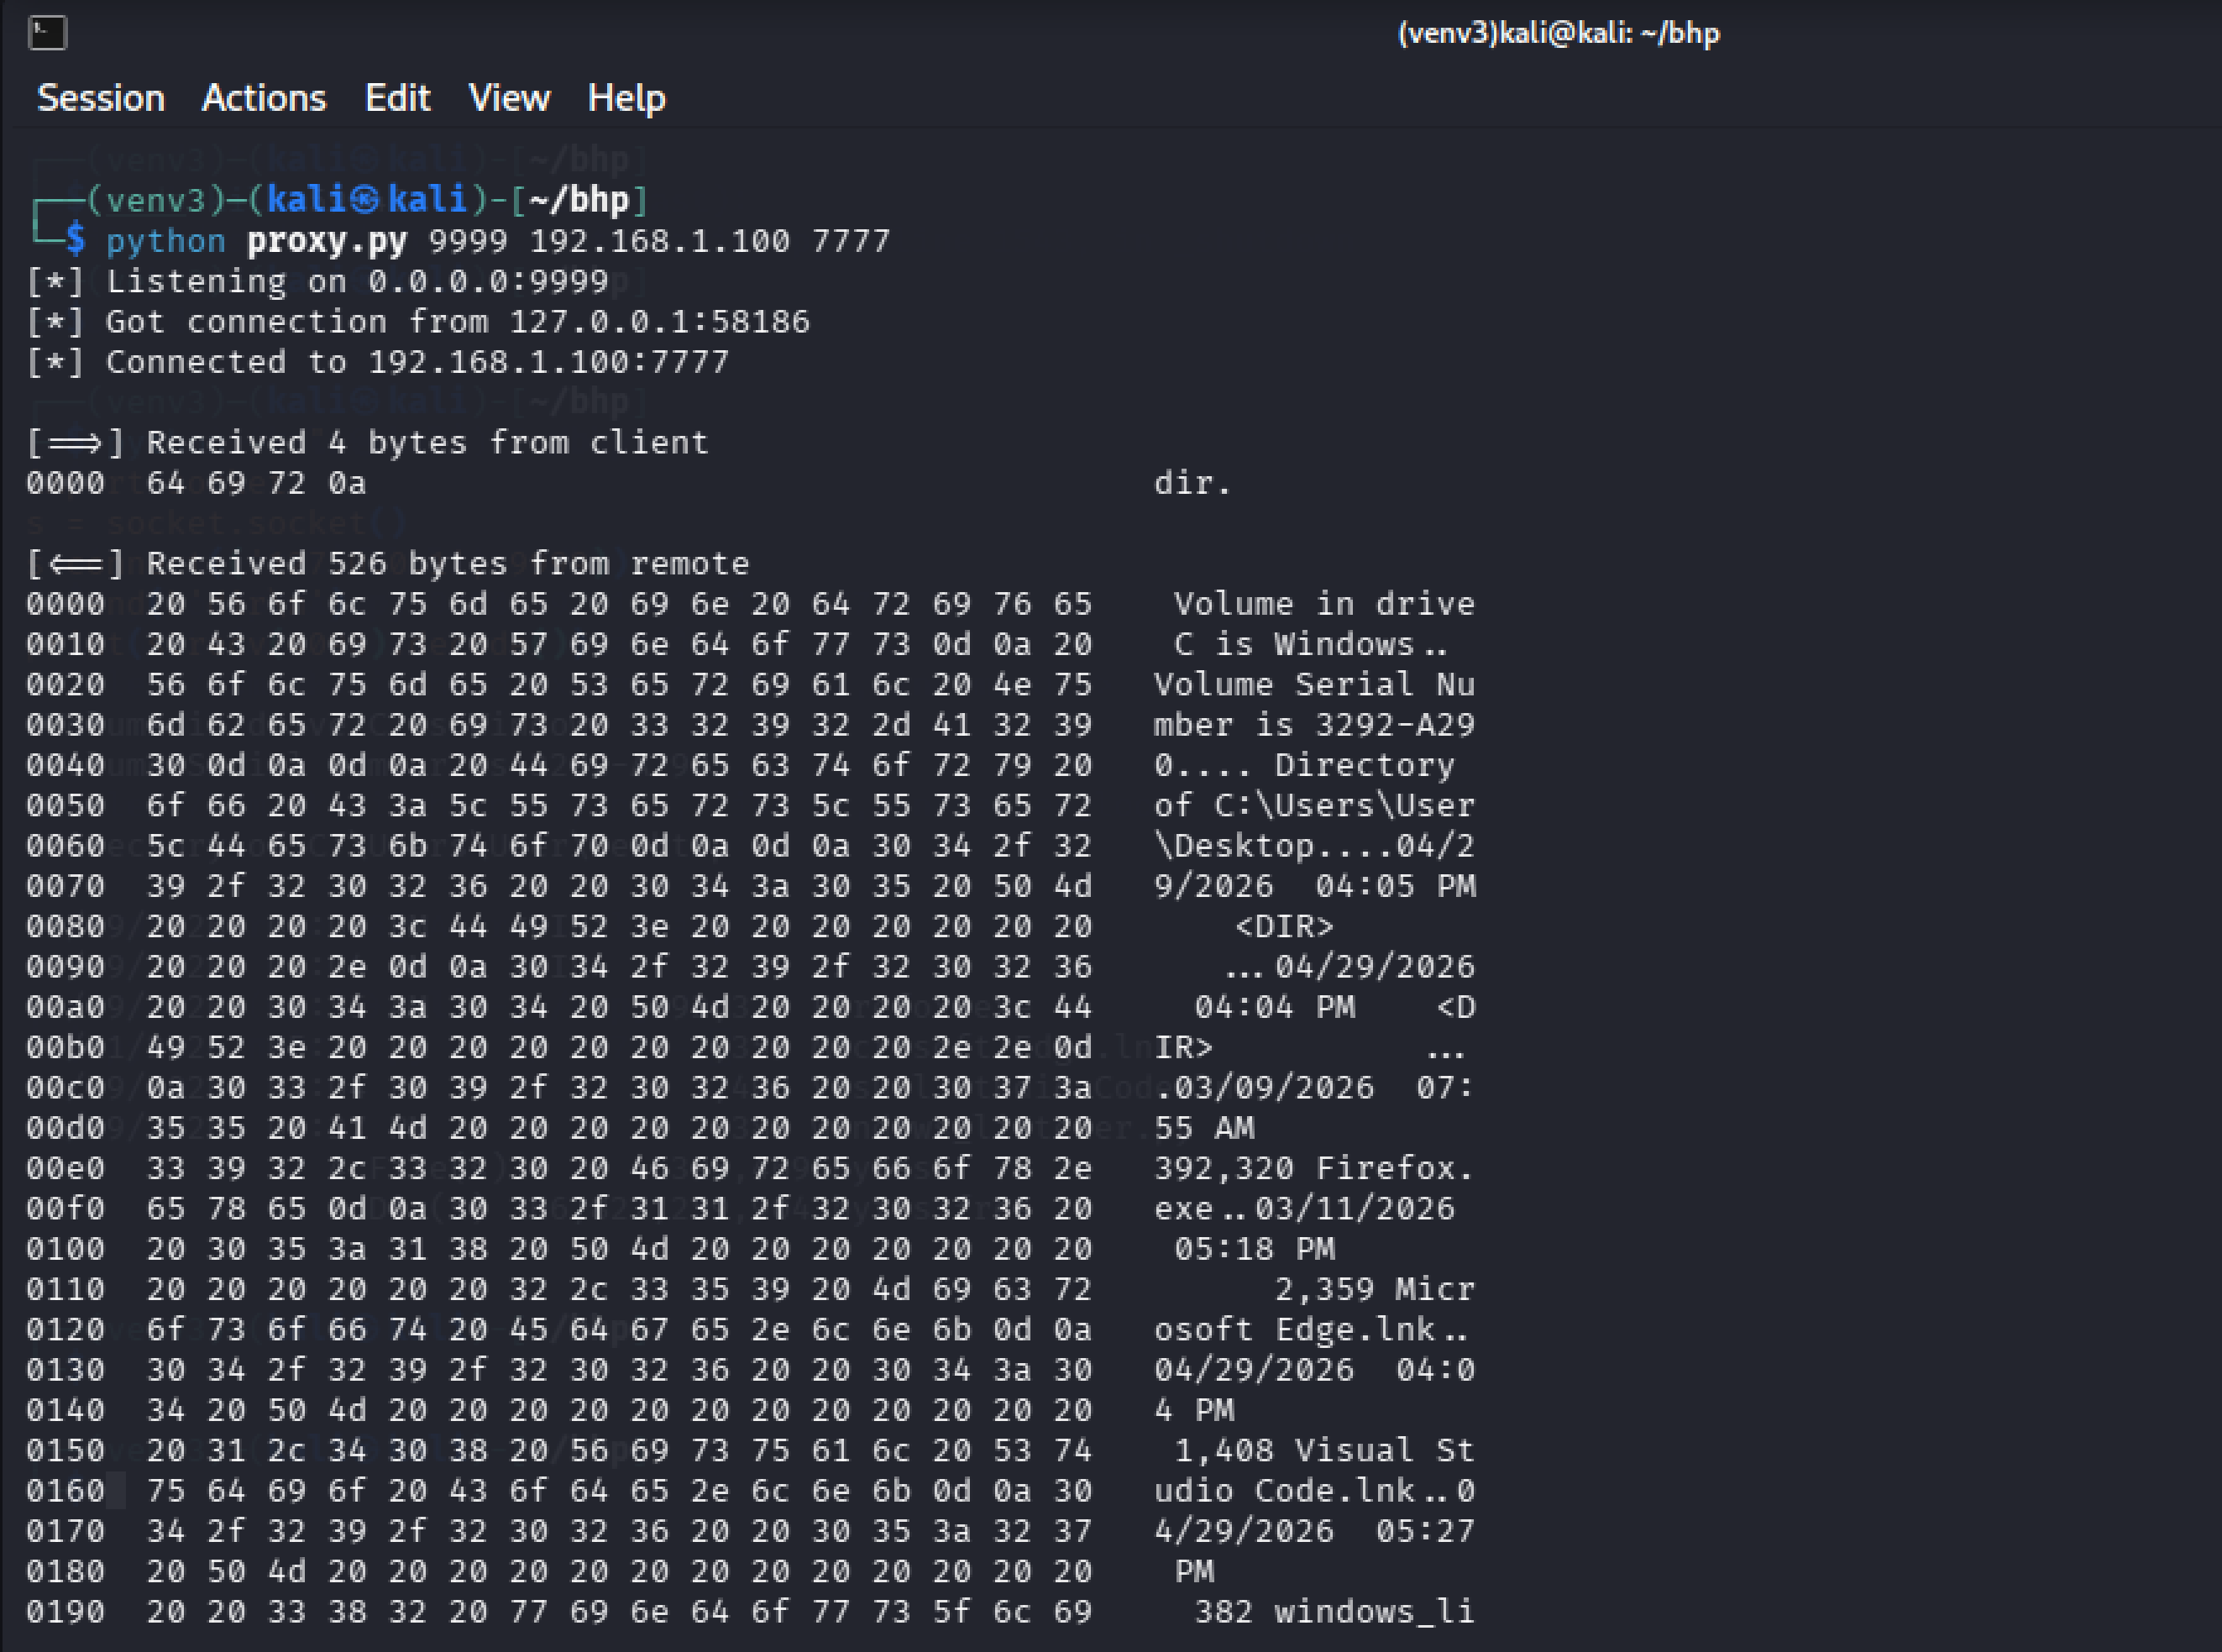
\includegraphics[width=0.5\textwidth]{mitm_attack.png}
    \caption{This is a screenshot of the data that was captured on the Windows machine during the MITM attack. 
    It was captured after running two commands, one to get the windows machine ready, and the other to pull 
    data onto the Linux Machine. The data that was captured was the output of the directory command, which 
    shows the volume for the drive, the serial number, applications installed, and the raw hexadecimal data.}
\end{figure}

\begin{figure}[h]
    \centering
    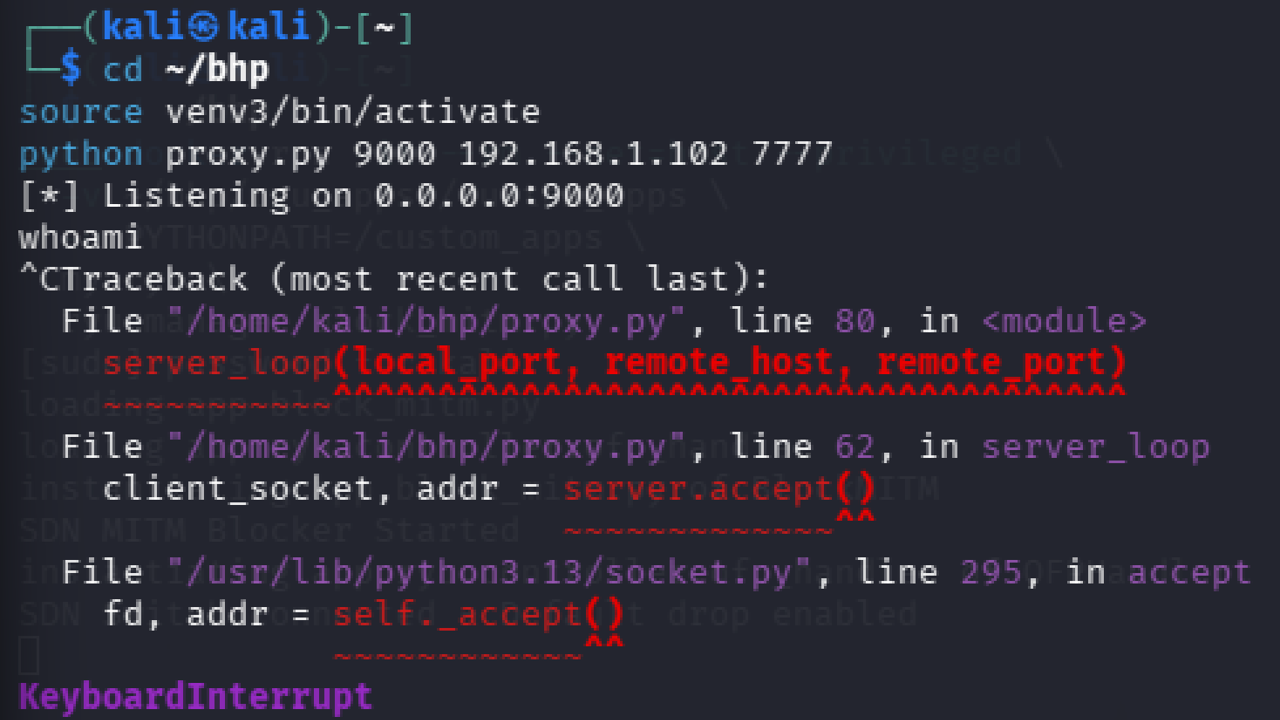
\includegraphics[width=0.5\textwidth]{MITM_Failure.png}
    \caption{This figure shows the output of the same attack type, same code, same virtual machines, but with 
    the implementation of an SDN in the network. As can be seen, the attack was not successful, and the 
    attacker was not able to capture any data from the Windows machine. This further shows the effectiveness 
    of the SDN in mitigating vulnerabilities in the home network.}
\end{figure}



\section{Conclusion}
Home networks remain dangerously vulnerable to attack, yet they receive far less attention in security 
research than enterprise networks. As noted in the introduction, 81\% of users never change their router's 
default admin username and password, and 79\% would not know how to change any settings if needed. This 
paper addressed this gap by simulating a typical home network using VirtualBox and comparing network 
security in a network without an SDN and with an SDN. A man in the middle (MITM) attack using ARP spoofing 
was executed against both configurations. 
The MITM attack succeeded on the average home network, capturing directory listing, application names, and 
raw hexadecimal data from the Windows 10 victim machine. As shown in Figure 1. When the same attack was 
attempted after implementing an SDN controller, the attack was completely mitigated. The controller, 
programmed with a simple policy, allowed only the routers MAC address to reply to ARP requests, mitigating 
the ARP poisoning attack before packets could reach the victim. Figure 2 shows how the attack had to be 
stopped after five minutes due to getting nothing from the network. This demonstrated the separation between 
the control plane and the data plane in the network, which is a core feature of an SDN, enabling security 
policies that are impossible in the traditional home network setup.
This study however did have its limitations. The network was simulated entirely in VirtualBox and was not 
deployed on physical hardware with real internet traffic. Additionally, only one type of attack was tested 
(ARP Spoofing). In future work, examining how an SDN controller can mitigate other types of attacks such as 
DNS spoofing or DDos attacks could be beneficial in understanding how they could make a home network more 
secure. This could all be done in an existing home network with the addition of a Raspberry Pi. Despite 
these limitations, this paper has clearly demonstrated the effectiveness of the SDN in mitigating MITM 
attacks in the home network setting. For the average user, the first step should be changing the default 
router username and password, the next best step is setting up an SDN to mitigate attacks that have made 
it into the network. For those who are looking to do so, a Raspberry Pi running OpenVSwitch could be a 
cheap and easy way to start securing their own network.
The implications of this study could extend beyond the specific MITM attack tested. If the SDN controller 
can become a more affordable and user-friendly device, they could become as common as home routers are today. 
A plug-and-play SDN device could be implemented in a next gen router and then could automatically enforce 
security policies on a home network that currently would require a lot of configuration. While this study 
used a simulation, the underlying principles apply to real world hardware. The same Open vSwitch and 
controller software tested here can run on a Raspberry Pi device costing less than one hundred dollars, 
making security accessible to home users ready to implement real security in their networks. 

\section{Addendum: The Use of Artificial Intelligence}
Generative AI tools were used in a limited and supporting way throughout the writing of this paper. 
Their use was restricted to brainstorming, clarification of technical concepts, finding sources, and 
formatting of the Methodology section. The actual MITM attack script used in this study was adapted 
directly from the Black Hat Python. 
When looking at difficult code examples, ChatGPT was occasionally used to describe what the code was 
doing in the given context, closely relating to how one would use the website Stack Overflow. Most 
prompts were used to ask technical questions relating to error messages from a Windows terminal. At 
no point was AI used in any way that would be against the Wooster Ethic.


\bibliographystyle{acm}
\bibliography{bibliography.bib}

\end{document}
